\chapter{Conclusion and Outlook}
There is still an ongoing discussion about the feasibility of \textit{Incoherent Diffractive Imaging} and its potential advantages over already established methods. It has not yet been experimentally proven that the assumptions made about the statistics of inner shell fluorescence are valid at the atomic level. Under the assumption of chaotic light, classical wave theory can illustrate the basic working principle.  In the quantum mechanical description of the underlying two-photon interference, indistinguishability between the quantum paths leading from the emission of two photons to simultaneous detection in two detectors creates the spatial bunching in the fluorescence patterns. Both explanations predict that a successful IDI experiment has to be designed with few distinguishable paths or modes.

The present work contributes simulations to validate theoretical considerations about the Signal-to-Noise characteristics and to optimize the experimental setup. Furthermore, previously published results indicating that IDI can extract spatial information out of X-ray fluorescence intensity patterns were validated.

\paragraph{Developed tools for IDI Experiments}
Both the GPU-accelerated simulation code and the reconstruction code developed for this thesis are open source\footnote{available under \url{https;//github.com/fzimmermann89/idi}}, and will be used for planning and analyzing future IDI experiments. The simulation allows a comparison of different samples and experimental setups with regards to the number of modes reducing the signal and the noise present in the measurement, as shown in \fref{chap:simulation}.
The analysis code implements 2D, 3D, and radial correlations for small and wide-angle experiments with different normalization approaches. Furthermore, it contains a library of commonly needed auxiliary functions, such as dark and mask generation for pixel detectors, a new common-mode correction with adaptive block sizes, photon counting procedures, different regression tools, and tools for center finding similar tasks.
Additionally, the developed alignment tool allows easy analysis of the detector orientation based on observed Kossel lines and will be used in future experiments with strict alignment margins.

\paragraph{Experimental Results}
The focal width of the FEL in vertical direction was successfully measured using IDI. The measurement was validated, first, by observing that the measured width increases as the sample is moved out of focus, and, second, by an independent wire scan measurement. Thus, the previously published results could be reproduced \cite{nakumura2020,inoue2019}. By detecting the fluorescence perpendicular to the FEL beam, in contrast to previous experiments, it was shown that the observed intensity correlations indeed stem from the fluorescence and not from coherent scattering.  The experiments using nanoparticle and crystal samples have been inconclusive so far. Thus, the proof of high-resolution imaging using IDI is still outstanding, and further refinements in the experimental design are necessary.


\paragraph{Experimental Improvements}
Recently, we performed an experiment using sub-1\,fs pulses at the CXI beamline at the LCLS free-electron laser \cite{subfs2017,argosecond}).
In this experiment, three major improvements over the SACLA experiment were implemented: First, the shorter pulse length reduces the number of temporal modes, and a shot-by-shot high-resolution spectrometer allows for better filtering of the X-ray pulses by estimated pulse length and intensity. Second, the data was recorded in forward direction, solving the undersampling issue and reducing the spatio-temporal modes due to the sample thickness. Finally, two new signal optimized samples were chosen. Anodic aluminum oxide (AAO) membranes with regular spaced 20\,nm or 30\,nm wide pores were filled with Nickel or Vanadium using atomic layer deposition, creating an array of hexagonal placed 500\,nm long cylinders 60\,nm/100\,nm apart \cite{carina2019}.  An exemplary SAXS measurement is shown in \fref{fig:saxsaao}. The other samples were lithographically produced nanogratings with two different pitches, 60\,nm  and 80\,nm \cite{mojarad2015}. Both types of samples combine the advantages of a single crystal sample (namely intense features) while providing more signal and requiring less accessible reciprocal space.  Simulations for both types of samples are shown in a  in \fref{fig:outlook_aao} and \fref{fig:outlook_grating}, respectively.
Based on these simulations, it can be estimated that a few hundred images taken with sub-fs pulses exciting 20\% of the atoms would suffice to reach an SNR of $>$5.
We were able to record complete datasets on multiple samples. The data analysis of this experiment has not yet been completed and might result in the first experimental proof of using fluorescence intensity correlation for structural imaging at the nanoscale.  


\paragraph{Using Incoherent Imaging for Online Beam Diagnostic}
Extending the results obtained for both determining the focal volume, as well as using the contrast to estimate the pulse length, promises to be a useful diagnostic tool in future FEL experiments with ultra-short pulses and/or tight foci \cite{nakumura2020,inoue2019}. In the aforementioned LCLS experiment, this has already been used successfully during tuning to find the focal spot along the beam direction. See \fref{fig:outlook_vanadium} for examples of the online analysis.

\paragraph{Higher Order Correlations}
Extending the Hanbury Brown and Twiss experiment to higher-order correlations allows the usage of prior knowledge about the distribution of the spatial frequencies in the sample. This provides an effective filter by fixing some terms in the correlation function at certain positions termed \textit{Magic Positions} \cite{schneider2018,thiel2007}. A future application of this scheme in analyzing the already recorded fluorescence patterns might lead to a significant increase in the SNR.

\vspace{0.5cm}
Overall, the results presented in this work have already led to improvements in the experimental design. Furthermore, there are possibilities for further improvements in the data analysis. Taken together, these improvements could result in a successful proof of principle experiment showing nanoscale resolution. Currently, IDI can already be used for diagnostics during FEL experiments
\clearpage
\vspace*{-1.5cm}
\begin{figure}[H]
	\centering
	\begin{subfigure}[b]{0.50\textwidth}
		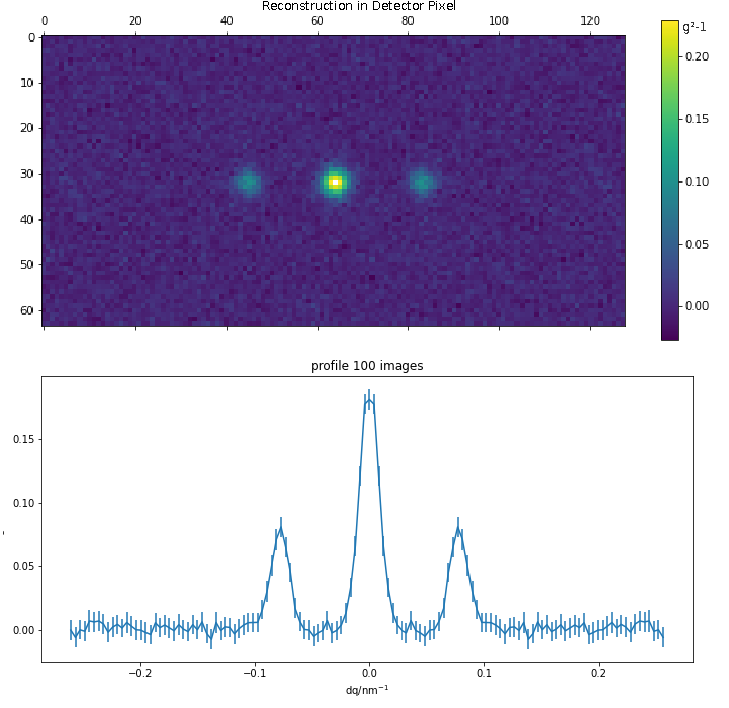
\includegraphics[width=\linewidth]{images/lv65simA.pdf}
		\caption{Nano-Grating}
		\label{fig:outlook_grating}
	\end{subfigure}
	\begin{subfigure}[b]{0.37\textwidth}
		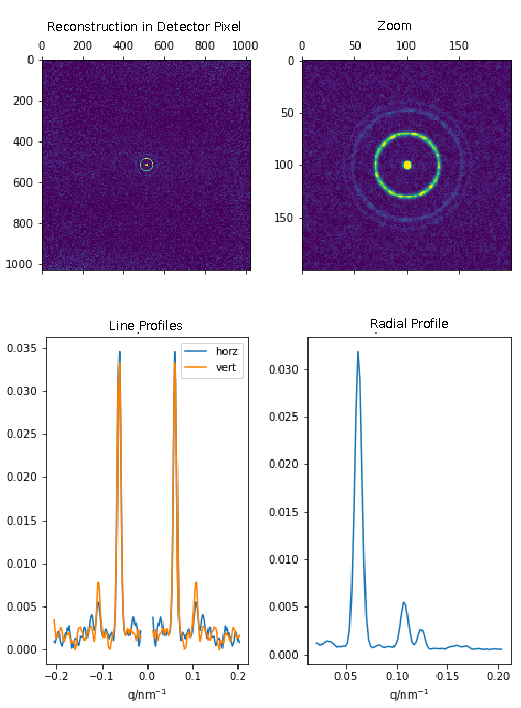
\includegraphics[width=\linewidth]{images/lv65simB.pdf}
		\caption{AAO membrane }
		\label{fig:outlook_aao}
	\end{subfigure}
	\caption[Simulations in preparation of LCLS experiment]{Examples of simulations performed with the tools developed in this thesis in preparation of the LCLS experiment LV65, which used nano-gratings and AAO membranes with metal-filled self-organized pores as samples for an IDI measurement. The simulations were performed optimize the sample geometry and to estimate the expected SNR. The images shown are the calculated fluorescence intensity correlations between pixels of a quarter of a Jungfrau 4M detector, placed at a distance of 70\,cm (grating) and 1\,m (membrane), respectively. The simulated grating has a pitch of 80\,nm, 40\,nm line width and 40\,nm thickness. The AAO membrane has an inter pore distance 105\,nm and the pores are filled with vanadium. Excitation of 20\% of the atoms and 4 modes was simulated. For both samples, an average of 100 images is shown. The features in the structure factors are much stronger, and a few hundred images should suffice for successful proof-of-principle experiment.}
\end{figure}
\vspace{-0.5cm}
\begin{figure}[H]
	\centering
	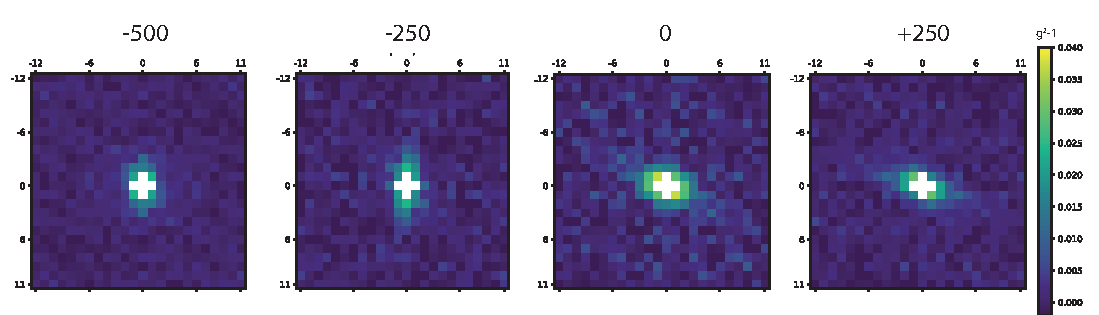
\includegraphics[width=\linewidth]{images/lv65_vanadium.pdf}	
	\caption[Focus finding using IDI]{Preliminary results of the $g^2(\vec{q})$ calculation of the fluorescence of a 4\,\textmu m vanadium foil, placed at 4 different positions along the X-ray beam at the CXI experimental hutch (LCLS). The beam was focus by \enquote{100 nm} KB optics (optimal theoretical focus size 90\,nm x 150\,nm, theoretical beam divergence 2 mrad x 1 mrad). One tile of a \textit{Jungfrau 4M} detector, placed 480\,mm downstream of the sample was used for the analysis. Shown are averages over 2000 shots with minimal shot-based filtering. The axes are in detector pixels. The position captioned \enquote{0\,\textmu m} was determined during the experiment as the focus based on these results, while the other positions are 250\,\textmu m and 500\,\textmu m further downstream and 250\,\textmu m upstream.  Most likely due to astigmatism, the extent of the focus in reciprocal space is larger, corresponding to a tighter focus, in vertical direction at -250\,\textmu m and in horizontal direction at +250\,\textmu m. The overall smallest focus is visible at 0\,\textmu m, resulting in the highest maximum amplitude of $g^2$.}
	\label{fig:outlook_vanadium}
\end{figure}

